\documentclass[12pt]{article}

\usepackage{url,verbatim, amsmath, amssymb, amsfonts, dsfont}
\usepackage{xcolor}
\usepackage{caption}
\captionsetup[figure]{font={color=red}}
\usepackage{graphicx}
\textwidth 15true cm
\textheight 9true in
\oddsidemargin 0.30true in
\evensidemargin 0.30true in
\topmargin -0.3true in
\headsep 0.4true in

\def\sgn{{\rm sign}}
\def\drightarrow{{\stackrel{d}{\rightarrow}}}
\def\dotsim{\stackrel{.}{\sim}}
\def\goesd{\stackrel{d}{\rightarrow}}
\def\goesp{\stackrel{p}{\rightarrow}}
\def\goeslaw{\stackrel{{\cal L}}{\longrightarrow}}
%
\def\vp{{\varphi}}
\def\E{{\rm E}}
\def\Pvalue{{$p$-value}}
\def\Pvalues{{$p$-values}}
\def\pr{{\rm pr}}
\def\Pr{{\rm pr}}
\def\logit{{\rm logit}}
\def\T{{ \mathrm{\scriptscriptstyle T} }}
\def\diag{{\rm diag}}  
\def\half{{\textstyle{1\over 2}}}
\def\ith{{$i{\rm th}$ }}
\def\var{{\rm var}}
\def\cl{{{\rm c}\ell}}
\def\checkx{{\checked\hspace{-6pt}\setminus}}
\def\grad{{\nabla}}

\sloppy %permits line-breaking of urls

\def\blue{\color{blue}}
\def\red{\color{red}}
\def\sgn{{\rm sign}}
\def\drightarrow{{\stackrel{d}{\rightarrow}}}

\usepackage{fancyhdr}
\pagestyle{fancy}
\fancyhf{} % clear default header/footer
\rhead{Ian Zhang \\ 1008367955} % your name on the left
\lhead{STA2212 HW1}  % page number on the right
\renewcommand{\headrulewidth}{0.4pt} % header line (set 0pt to remove)


\begin{document}

\noindent{\bf Questions Week 1} {\hfill STA 2212S 2026}\\

%{\bf Due January 14} \hfill{\it MS, Exercise 5.2}

\bigskip

\begin{enumerate}

\item  Suppose $(X_1, Y_1),  \dots, (X_n, Y_n)$ are independent pairs of random variables where $X_i$ and $Y_i$ are i.i.d. $N(\mu, \sigma^2)$ random variables: $$ f(x_i;\mu, \sigma^2) = \frac{1}{\sqrt{2\pi}\sigma}\exp\{-\frac{1}{2\sigma^2}(x_i - \mu)^2\}; \quad 
f(y_i;\mu, \sigma^2) = \frac{1}{\sqrt{2\pi}\sigma}\exp\{-\frac{1}{2\sigma^2}(y_i - \mu)^2\}; \quad$$
\begin{description}
\item{(a)} 	  Find the maximum likelihood estimators $\hat\mu$ and $\hat\sigma^2$ of $\mu$ and $\sigma^2$. 
\item{(b)} Show that $\hat\sigma^2 \goesp \sigma^2$ as $n \rightarrow\infty$.
\item{(c)} Suppose now that each pair $(X_i, Y_i)$ has a different expected value, $\mu_i, i = 1, \dots, n$. Show that the maximum likelihood estimator $\hat\sigma^2 \goesp \sigma^2/2$ as $n\rightarrow\infty$. 
\item{(d)} Define $Z_i = X_i-Y_i$.  Find the maximum likelihood estimator of $\sigma^2$ based on $Z_1, \dots, Z_n$, and show that it converges in probability to $\sigma^2$.
\end{description}


\textcolor{red}{(a) Without loss of generality, consider the log-likelihood function of $(\mu, \sigma)$ based on the $X_1,\ldots, X_n$. 
\begin{equation*}
  \ell(\mu, \sigma \mid x_1,\ldots, x_n) \propto -n\log \sigma - \sum_{i=1}^n \frac{1}{2\sigma^2}(x_i - \mu)^2
\end{equation*}
We compute partial derivatives of $\ell$ with respects to $\mu$ and $\sigma$, and set them to 0 to obtain the MLE of the parameters. 
\begin{align*}
  \frac{\partial \ell}{\partial \mu} &= \sum_{i=1}^n \frac{1}{\sigma^2}(x_i - \mu) = 0\\
  \frac{\partial \ell}{\partial \sigma} &= -\frac{n}{\sigma^2} + \sum_{i=1}^n \frac{1}{\sigma^3} (x_i - \mu)^2 = 0 
\end{align*}
Solving these equations yields 
\begin{equation*}
  \hat \mu = \frac1n \sum_{i=1}^n X_i \qquad \hat \sigma^2 = \frac{1}{n}\sum_{i=1}^n (x_i - \mu)^2 = \frac{1}{n}\sum_{i=1}^n (X_i - \bar X)^2
\end{equation*}
(b) By the weak law of large numbers and continuous mapping theorem, 
\begin{align*}
  \hat\sigma^2 &= \frac1n \sum_{i=1}^n (X_i - \bar X)^2\\
  &= \frac{1}{n}\left(\sum_{i=1}^n X_i^2 - n \bar X^2\right)\\
  &= \overline{X^2} - \bar X^2\\
  &\stackrel{p}{\to} E(X_1^2) - \mu^2\\
  &= \sigma^2 + \mu^2 - \mu^2\\
  &= \sigma^2
\end{align*}
as required. \\
(c) Consider the log-likelihood
\begin{equation*}
  \ell(\mu_1,\ldots, \mu_n, \sigma^2 \mid x_1,\ldots, x_n, y_1,\ldots, y_n) \propto -n\log\sigma - \sum_{i=1}^n \frac{1}{2\sigma^2} ((x_i - \mu_i)^2 + (y_i - \mu_i)^2)
\end{equation*} 
For each $i$, 
\begin{equation*}
  \frac{\partial \ell}{\partial \mu_i} = \frac{1}{\sigma^2}(x_i + y_i - 2\mu_i) 
\end{equation*}
Setting each to 0 yields an MLE 
\begin{equation*}
  \hat\mu_i = \frac{1}{2}(X_i + Y_i)
\end{equation*}
The partial derivative of $\ell$ with respects to $\sigma$ is 
\begin{equation*}
  \frac{\partial \ell}{\partial \sigma} = -\frac{n}{\sigma} + \frac{1}{\sigma^3}\sum_{i=1}^n ((x_i - \mu_i)^2 + (y_i - \mu_i)^2)
\end{equation*}
Setting this to 0 yields the MLE 
\begin{equation*}
  \hat\sigma^2 = \frac{1}{n}\sum_{i=1}^n [(X_i - \hat\mu_i)^2 + (Y_i - \hat \mu_i)^2] = \frac{1}{2n} \sum_{i=1}^n (X_i - Y_i)^2
\end{equation*}
Let $Z_i = X_i - Y_i$, so the $Z_i$ are i.i.d. $\mathcal N(0, \sigma^2)$. Then by the WLLN and continuous mapping theorem, 
\begin{equation*}
  \hat\sigma^2 = \frac{1}{2n} \sum_{i=1}^n Z_i^2 \stackrel{p}{\to} \frac{1}{2}(E(Z_1^2)) = \frac{1}{2} (0 + \sigma^2) = \frac{\sigma^2}{2}
\end{equation*}
as required. \\
(d) Since the $Z_i$ are i.i.d. $\mathcal N(0, \sigma^2)$, the log-likelihood function of $\sigma$ is given by 
\begin{equation*}
  \ell (\sigma \mid z_1,\ldots, z_n) \propto -n \log \sigma - \sum_{i=1}^n \frac{1}{2\sigma^2}z_i^2
\end{equation*}
thus the partial derivative of $\ell$ with respects to $\sigma$ is 
\begin{equation*}
  \frac{\partial \ell}{\partial \sigma} = -\frac{n}{\sigma} + \frac{1}{\sigma^3} \sum_{i=1}^n z_i^2
\end{equation*}
Setting the above to 0 yields the MLE 
\begin{equation*}
  \hat\sigma^2 = \frac{1}{n}\sum_{i=1}^n Z_i^2 = \frac{1}{n}\sum_{i=1}^n (X_i - Y_i)^2
\end{equation*}
To show consistency, we use the WLLN and continuous mapping theorem again: 
\begin{equation*}
  \hat\sigma^2 = \frac{1}{n}\sum_{i=1}^n Z_i^2 = \overline{Z^2} \stackrel{p}{\to} E(Z_1^2) = \sigma^2
\end{equation*}
as required. 
}

\item Suppose $X_1, \dots, X_n$ are independent and identically distributed normal random variables with expected value $\theta$ and variance 1. %: $$ f(x;\theta) = \frac{1}{\surd{2\pi}}\exp\{-\frac{1}{2}(x - \theta)^2.$$
Define $$
Y_{i} =
    \begin{cases}
      1 & \text{if $X_i > 0$} \\
      0 & \text{if $X_i \le 0$}.
    \end{cases}       
$$
Let $\psi = \text{Pr}(Y_i = 1)$.
\begin{description}
\item{(a)} 	  Find the likelihood function for $\theta$ based on $X_1, \dots, X_n$, and show that the maximum likelihood estimator of $\theta$ is $\hat\theta = \bar X$.  Express $\psi$ as a function of $\theta$ and hence compute an expression for the maximum likelihood estimator of $\psi$. 
\item{(b)} Find the approximate variance of $\hat\psi$ using the delta method.
\item{(c)} Define $\tilde\psi = \frac{1}{n}\sum_{i=1}^n Y_i$. Show that $\tilde\psi$ is a consistent estimator of $\psi$. 
\item{(d)} Compute the asymptotic relative efficiency of $\tilde\psi$ to $\hat\psi$. This is defined as the asymptotic variance of $\hat\psi$ divided by the asymptotic variance of $\tilde\psi$; see \S 9.8. The answer is a function of $\theta$.
\item {(e)} Plot the asymptotic relative efficiency for $\theta\in (-5, 5)$.
\item{Comment}: These calculations are extended to the regression setting in SM \S 10.4.1, Ex. 10.17, where they are used to study the loss of information in converting a continuous response to a binary response.  
\end{description}
\textcolor{red}{
  (a) The likelihood function is given by 
  \begin{equation*}
    \mathcal L(\theta \mid x_1, \ldots, x_n) \propto \prod_{i=1}^n \exp\left(-\frac{1}{2}(x_i - \theta)^2\right) = \exp\left(-\frac{1}{2}\sum_{i=1}^n (x_i - \theta)^2 \right)
  \end{equation*}
  The log-likelihood is thus 
  \begin{equation*}
    \ell (\theta \mid x_1,\ldots, x_n) \propto -\frac{1}{2}\sum_{i=1}^n (x_i - \theta)^2
  \end{equation*}
  so the partial derivative of $\ell$ with respects to $\theta$ is 
  \begin{equation*}
    \frac{\partial \ell}{\partial \theta} = \sum_{i=1}^n (x_i - \theta)
  \end{equation*}
  Setting the above to 0 yields the MLE 
  \begin{equation*}
    \hat\theta = \bar X
  \end{equation*}
  By definition of $\psi$,
  \begin{equation*}
    \psi = \text{Pr}(Y_i = 1) = \text{Pr}(Y_1 = 1) = \text{Pr}(X_1  > 0) = \Phi(\theta)
  \end{equation*}
  where $\Phi$ is the CDF of a standard Gaussian random variable. This yields an MLE 
  \begin{equation*}
    \hat \psi = \Phi(\hat\theta) = \Phi (\bar X)
  \end{equation*}
  (b) By the CLT, we know 
  \begin{equation*}
    \sqrt n(\hat\theta - \theta) = \sqrt n(\bar X - \theta) \stackrel{d}{\to} \mathcal N(0, 1)
  \end{equation*}
  By the Delta method, since $\Phi$ is continuously differentiable at $\theta$ with nonzero derivative $\phi(\theta)$ at all $\theta \in \mathbb R$, we have 
  \begin{equation*}
    \sqrt n(\hat\psi - \psi) \stackrel{d}{\to} \phi'(\theta)\mathcal N(0, 1) = \mathcal N(0, (\phi'(\theta))^2)
  \end{equation*}
  thus the asymptotic variance is $n^{-1}(\phi' (\theta))^2$. \\
  (c) By the WLLN, 
  \begin{equation*}
    \tilde \psi \stackrel{p}{\to} E(Y_1) = \text{Pr}(Y_1 = 1) = \psi
  \end{equation*}
  (d) By the CLT,
  \begin{equation*}
    \sqrt n (\tilde \psi - \psi) \stackrel{d}{\to} \mathcal N(0, \text{Var}(Y_1))
  \end{equation*}
  where the variance of $Y_1$ is computed as 
  \begin{equation*}
    \text{Var}(Y_1) = \psi(1 - \psi)
  \end{equation*}
  So, the variance of $\tilde \psi$ is $n^{-1} \psi(1 - \psi)$. 
  The ARE is thus 
  \begin{equation*}
      \text{ARE}(\tilde \psi, \hat \psi) = \frac{(\phi'(\theta))^2}{\Phi(\theta)\Phi(-\theta)}
  \end{equation*}
  (e) \begin{figure}[h]
  \centering
  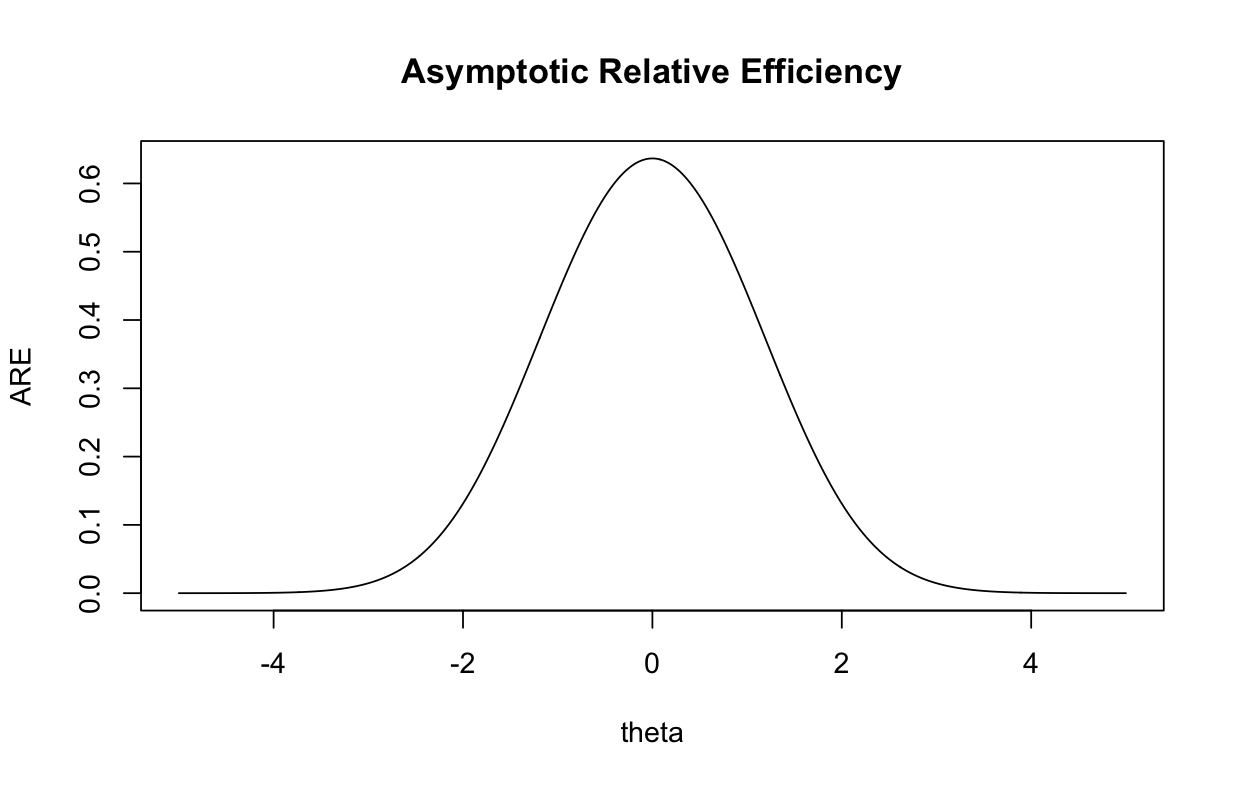
\includegraphics[width=0.75\textwidth]{STA2212_HW1_ARE_plot.png}
  \caption{\textcolor{red}{Asymptotic relative efficiency of $\tilde{\psi}$ to $\hat{\psi}$ for $\theta \in (-5,5)$.}}
  \label{fig:are-plot}
\end{figure}
}


\end{enumerate}
\end{document}

